\makeatletter
\def\input@path{{../../}}
\makeatother
\documentclass[../../main.tex]{subfiles}

\graphicspath{
	{../../img/}
	{../img/}
	{img/}
}

\begin{document}
	\subsection{Связь КрИ-2 и КрИ-1}
	
	Пусть задана кривая:
	\[
	\begin{cases}
	x = x(t),\\
	y = y(t),\\
	\alpha \leq t \leq \beta.
	\end{cases}
	\]
	
	\begin{center}
		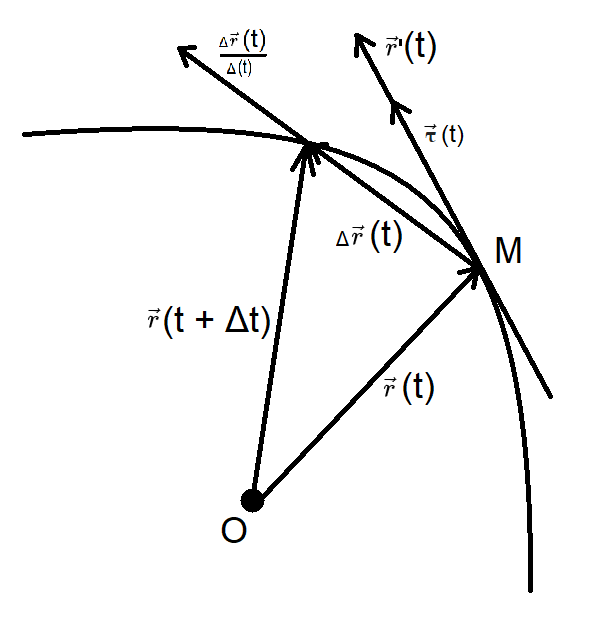
\includegraphics[scale = 0.8]{lec20_1.png}
	\end{center}
	
	Тогда:
	\begin{gather*}
	\vec r(t) = \left( x(t), y(t) \right) \\
	\vec r\,'(t) = \left( x'(t), y'(t) \right)
	\end{gather*}
	
	Если $\Delta t \to 0$, то $\frac{\Delta \vec{r}}{\Delta t}$
	$ \appr{\Delta t \to 0}
	\vec{r}\,'(t)$.
	Если $\Delta \vec{r} \to 0$, то $N$ приблизится к $M$
	и займет свое предельное положение.
	$\frac{\Delta \vec{r}}{\Delta t}$ также изменится и займет 
	свое предельное положение~--- касательный вектор кривой в точке $M$. Его 
	длина:
	
	\[
	\abs{\vec r\,'} =
	\sqrt{\left( x'(t) \right)^2 + \left( y'(t) \right)^2}.
	\]
	
	Если рассматривать $\vec{\tau} = 
	\dfrac{\vec{r}\,'(t)}{\abs{\vec{r}\,'}}$, то
	$\vec{\tau}$~--- касательный вектор, сонаправленный
	с $\vec r\,'$,
	но при этом $\abs{\vec{\tau}} = 1$. То есть,
	$
	{\vec{\tau}} = (\cos\alpha, \cos\beta)
	$,
	где $\alpha, \beta$~--- углы, образованные вектором $\vec{\tau}$
	или $\vec{r}\,'$ с положительными координатными полуосями
	$Ox$ и $Oy$ (соответствующие направляющие косинусы векторов
	$\vec{\tau}$ или $\vec{r}\,'$).
	
	Отсюда имеем:
	\begin{gather*}
	\vec{r}\,'(t) = \vec{\tau}(t)\abs{\vec{r}\,'(t)} 
	=
	(\abs{\vec{r}\,'(t)}\cos \alpha,\ \abs{\vec{r}\,'(t)}\cos 
	\beta)
	\implies\,
	\\
	\implies\, \begin{cases}
	x'(t) = \abs{\vec{r}\,'(t)}\cos \alpha\, \\
	y'(t) = \abs{\vec{r}\,'(t)}\cos \beta\,
	\end{cases} \implies
	\begin{cases}
	dx = \abs{\vec{r}\,'(t)} dt\cdot\cos \alpha\, \\
	dy = \abs{\vec{r}\,'(t)} dt\cdot\cos \beta\,
	\end{cases}
	\end{gather*}
	
	Если зафиксировать некоторое $t$, то этому значению
	на кривой соответствует точка,
	которой соответствует значение параметра $S$:
	\[
	t \longleftrightarrow M(t) \longleftrightarrow S\, 
	\text{~--- длина кривой от точки}\, A.
	\]
	
	Естественная параметризация кривой:
	\begin{gather*}
	S = S(t) = \int\limits_{\alpha}^{t} \sqrt{\left( x'(t) \right)^2
	+ \left( y'(t) \right)^2}\, dt.
	\implies [\text{теорема Барроу}] \implies
	\\ \implies
	S'(t) = \sqrt{\left( x'(t) \right)^2 + \left( y'(t) \right)^2}\, =
	\abs{\vec{r}\,'(t)} \implies
	\abs{\vec{r}\,'}dt\, = S'dt\, = ds \implies \\
	\implies
	\begin{cases}
	dx = ds \cos \alpha\, = \cos \alpha\, ds, \\
	dy = ds \cos \beta\, = \cos \beta\, ds.
	\end{cases}
	\end{gather*}
	
	Поэтому
	\begin{equation}
	\label{lec_20, num_1}
	\int\limits_{\tiny{\overbow{AB}}} P \left( x(t),y(t) \right)\, dx + Q \left( 
	x(t), y(t)
	\right)\, dy =
	\int\limits_{\tiny{\overbow{AB}}} \left( P(x,y)\, \cos \alpha\,
	+ Q(x, y)\, \cos \beta \right)ds.
	\end{equation}
	
	Слева записан КрИ-2, справа~--- КрИ-1 по одной и той же кривой.
	
	\begin{rem}
		В КрИ-2 направлением на кривой $\overbow{AB}$~---
		является направление возрастания $t$,
		и косинусы соответствуют этому направлению.
	\end{rem}	
		
В случае КрИ-2 по произвольной кривой $\overbow{AB}$ в $\R^3$ имеем:
\[
\begin{gathered}
\int\limits_{\tiny{\overbow{AB}}} P \left(x, y, z \right)\, dx\,
+ Q \left(x, y, z \right)\, dy + R \left(x, y, z \right)\, dz\, = \\
= \int\limits_{\tiny{\overbow{AB}}} \left( P \left(x, y, z \right)\, \cos 
\alpha\,
+ Q \left(x, y, z \right)\, \cos \beta\, + R \left(x, y, z \right)\, \cos 
\gamma\, \right)ds,
\end{gathered}
\]
где $P, Q, R$ ~--- функции от $x, y, z$; $\cos \alpha, \cos \beta,
\cos \gamma$ ~--- направляющие косинусы касательного вектора
к $\overbow{AB}$.
	
	\begin{rem}
		Если кривая является кусочно-гладкой, т.~е. состоит из конечного множества 
		дуг,
		каждая из которых~--- гладкая кривая, то интеграл необходимо разбить, 
		используя
		свойство аддитивности.
	\end{rem}

\section{Формула Грина}

Пусть $D \subset \R^2$~--- некоторая область из $\R^2$, в которой
располагается замкнутая область $G \subset D$ с границей $L$.

Говорят, что на $L$ выбрано положительное направление,
если при движении в таком направлении область $G$ остается слева
(то есть движение происходит против часовой стрелки).

\begin{center}
	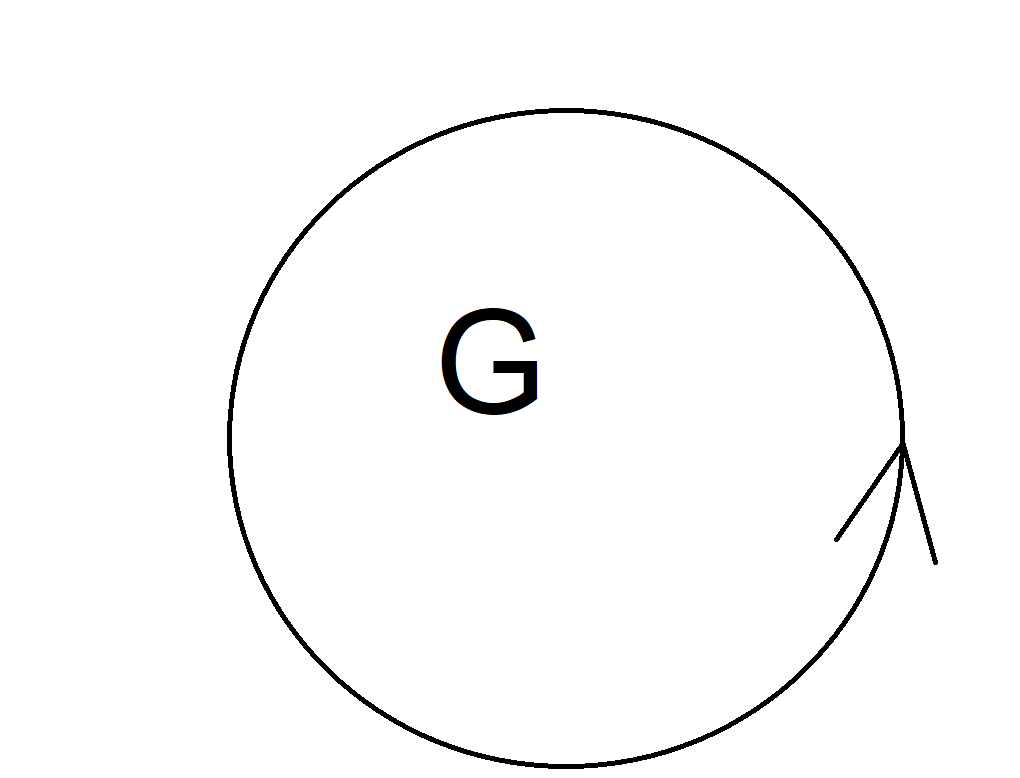
\includegraphics[scale = 0.4]{lec20_2.png}
\end{center}

\begin{thm}[формула Грина]
	Если функции $P$ и $Q$ непрерывны и имеют непрерывные частные производные 
	$P'_y, Q'_x$, то
	\begin{equation}
	\label{lec_20, num_2}
	\int\limits_{L} P( x, y)\, dx + Q( x, y)\,
	dy = \iint\limits_{G} \left( Q_x'(x, y)
	- P_y'(x, y) \right)\, dx\, dy,
	\end{equation}
	где $L$ пробегает в положительном направлении.
	
	(Слева находится КрИ-2, справа ~--- 2И.)
\end{thm}

\begin{proof}
	Рассмотрим
	\[
	- \iint\limits_{G} P_y'(x, y)\, dx\, dy.
	\]
	
	\begin{itemize}
		\item[а)] Область $G$ ограничена и является
		криволинейной трапецией ($AD$, $BC$~--- 
		вертикальные прямые):
		\begin{center}
			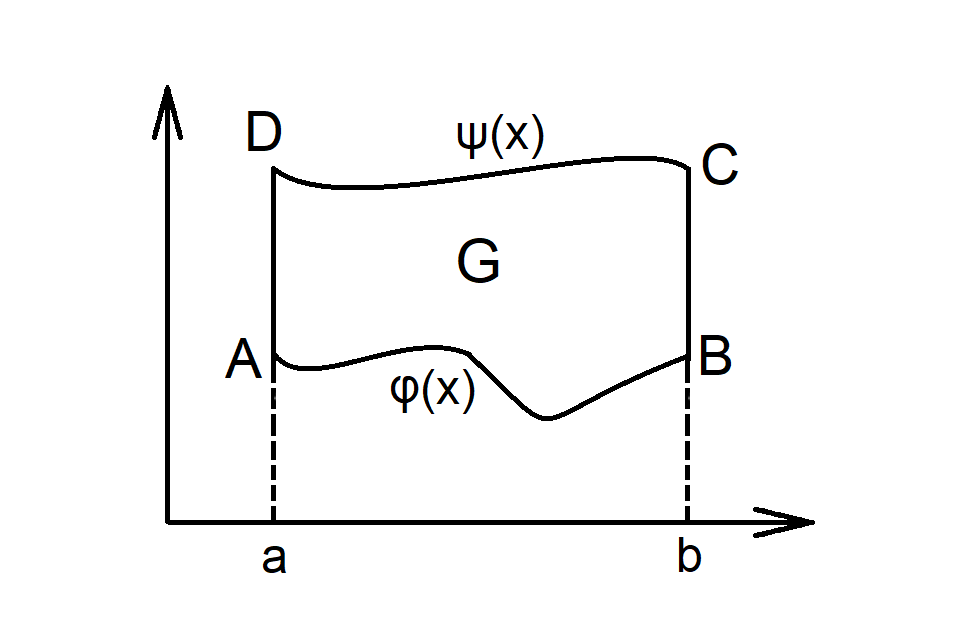
\includegraphics[scale = 0.5]{lec20_3.png}
		\end{center}
	
		Тогда
		\[
		\begin{gathered}
			- \iint\limits_{G} P_y'(x, y)\, dx\, dy =
			- \int\limits_{a}^{b}\, dx \int\limits_{\phi(x)}^{\psi(x)} P_y'
			(x, y)\, dy =
			- \int\limits_{a}^{b}\left(P(x, \psi(x))\, -
			P(x, \phi(x)) \right)\,dx = \\
			= \int\limits_{b}^{a} P(x, \phi(x))\,dx +
			\int\limits_{a}^{b} P(x, \psi(x))\,dx = 
			\int\limits_{\tiny{\overbow{AB}}} P(x, y)\,dx +
			\int\limits_{\tiny{\overbow{CD}}} P (x, y)\,dx = \\
			= \left[\int\limits_{\tiny{\overbow{BC}}} P (x, y)\,dx = 0,\ 
			\int\limits_{\tiny{\overbow{DA}}} P (x, y)\,dx = 0\right]	
			= \int\limits_{\tiny{\overbow{AB}}} P (x, y)\,dx +
			\int\limits_{\tiny{\overbow{CD}}} P (x, y)\,dx + \\
			+ \int\limits_{\tiny{\overbow{BC}}} P (x, y)\,dx +
			\int\limits_{\tiny{\overbow{DA}}} P (x, y)\,dx =
			\int\limits_{L} P (x, y)\,dx,
		\end{gathered}
		\]
		то есть
		\begin{equation}
		\label{lec_20, num_3}
		-\iint\limits_{G} P_y' (x, y)\, dx dy = 
		\int\limits_{L} P (x, y) dx.
		\end{equation}
		
		\item[б)] Если область $G$ имеет более сложную конфигурацию, ее разбивают
		на часть вида а) с помощью вертикальных отрезков и
		используют свойство аддитивности интегралов.
		Например:
		\begin{center}
			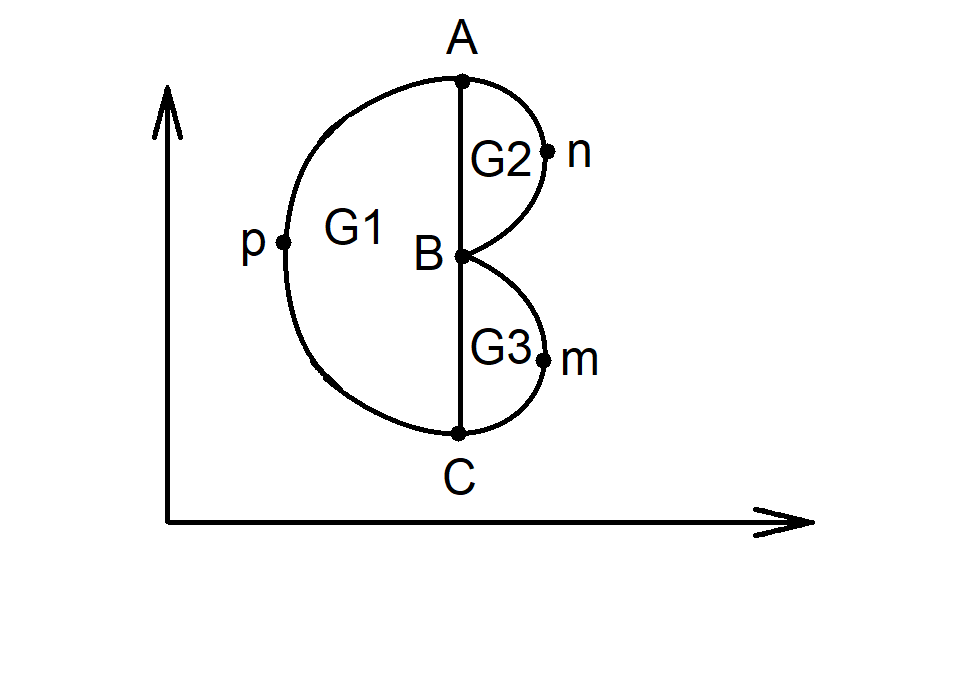
\includegraphics[scale = 0.8]{lec20_4.png}
		\end{center}
		\[
		\begin{gathered}
		\iint\limits_{G} = \iint\limits_{G_1} + \iint\limits_{G_2} +
		\iint\limits_{G_3} =
		\int\limits_{\tiny{\overbow{ApC}}} + \int\limits_{\tiny{\overbow{CB}}} +
		\int\limits_{\tiny{\overbow{BA}}} + \int\limits_{\tiny{\overbow{BnA}}} +
		\int\limits_{\tiny{\overbow{AB}}} + \int\limits_{\tiny{\overbow{CmB}}} +
		\int\limits_{\tiny{\overbow{BC}}} =
		\int\limits_{L}.
		\end{gathered}
		\]		
	\end{itemize}

	\bigskip
	
		Теперь рассмотрим
		\[
		\iint\limits_{G} Q_x' (x, y) dx dy.
		\]
		\begin{center}
			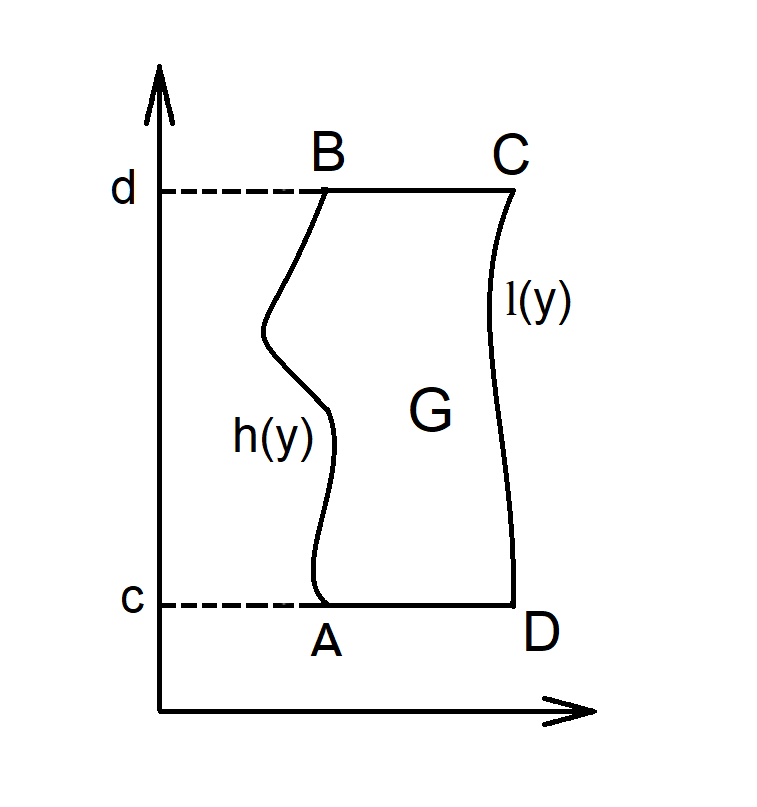
\includegraphics[scale = 0.6]{lec20_5.png}
		\end{center}
		
	\begin{itemize}
		\item[a)]
		\[
		\begin{gathered}
		\iint\limits_{G} Q_x' (x, y) dx dy =
		\int\limits_{c}^{d}\, dy \int\limits_{h(x)}^{l(x)} Q_x'
		(x, y)\, dx =
		\int\limits_{c}^{d}\, \left(Q (l(x), y)\, -
		Q (h(x), y) \right) dy = \\
		= \int\limits_{c}^{d} Q (l(x), y)\, dy +
		\int\limits_{d}^{c} Q (h(x), y)\, dy =
		\int\limits_{c}^{d} Q (l(x), y)\, dy +
		\int\limits_{d}^{c} Q (h(x), y)\, dy = \\
		\int\limits_{\tiny{\overbow{CD}}} Q (x, y)\, dy +
		\int\limits_{\tiny{\overbow{AB}}} Q (x, y)\, dy =
		\int\limits_{\tiny{\overbow{CD}}} Q (x, y)\, dy +
		\int\limits_{\tiny{\overbow{AB}}} Q (x, y)\, dy + \\ +
		\int\limits_{\tiny{\overbow{BC}}} Q (x, y)\, dy +
		\int\limits_{\tiny{\overbow{DA}}} Q (x, y)\, dy =
		\int\limits_{L} Q \left(x, y \right)\, dy.
		\end{gathered}
		\]
		
		\item[б)] Если $G$~--- область более сложной конфигурации, то ее
		разбивают на части вида а) с помощью горизонтальных отрезков и
		используют свойство аддитивности интегралов.
	\end{itemize}

Получаем
\begin{equation}
\label{lec_20, num_4}
\iint\limits_{G} Q_x' (x, y)\, dx\, dy =
\int\limits_{L} Q (x, y)\, dy.
\end{equation}

Сложив \eqref{lec_20, num_3} и \eqref{lec_20, num_4}, используя свойство 
линейности КрИ, получим 
\eqref{lec_20, num_2}.
\end{proof}

\subsection{Случай многосвязной области}

\begin{defn}
	Область $D$ называется \emph{односвязной}, если любую замкнутую кривую $L 
	\subset D$ 
	можно стянуть в точку, не выходя за пределы $D$.
\end{defn}

\begin{center}
	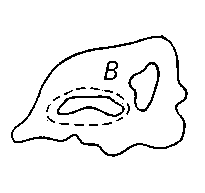
\includegraphics[scale = 1.5]{lec20_6.png}
\end{center}

Заштрихованная область является \emph{многосвязной}.

Пусть в \eqref{lec_20, num_2} $G$~--- многосвязная область. Формула 
справедлива
и в этом случае. Тогда ее граница $L$ пробегает в 
положительном направлении и
состоит из контуров $l_1, l_2, l_3$:
\begin{center}
	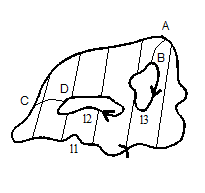
\includegraphics[scale = 1.5]{lec20_7.png}
\end{center}

Для доказательства соединим $l_2$, $l_3$ с $l_1$ с помощью гладких
спрямляемых кривых. Тогда область становится односвязной.

Граница состоит из кривых $\overbow{AC} \cup \overbow{CD} \cup l_2 \cup 
\overbow{DC} 
\cup \overbow{CA} \cup \overbow{AB} \cup l_3 \cup \overbow{BA} = L$

При обходе $L$ в положительном направлении кривые $\overbow{AB}$ и 
$\overbow{CD}$ пробегают дважды в противоположных направлениях, поэтому сумма 
интегралов по этим кривым дает $0$.
То есть, в КрИ-2 слева можно учитывать интегралы только по $l_1, l_2, l_3$.
В 2И справа величина интеграла не изменяется, так как кривые имеют нулевую 
площадь.

\begin{example}
	Вычислить $\displaystyle\int\limits_{\tiny{\overbow{AB}}} x^2 \cos y\, dx
	- \frac{x^3}{3}	\sin y\, dy,\  
	\text{по } \overbow{AB}:
	y = 3x - x^2.$
	
	\begin{center}
		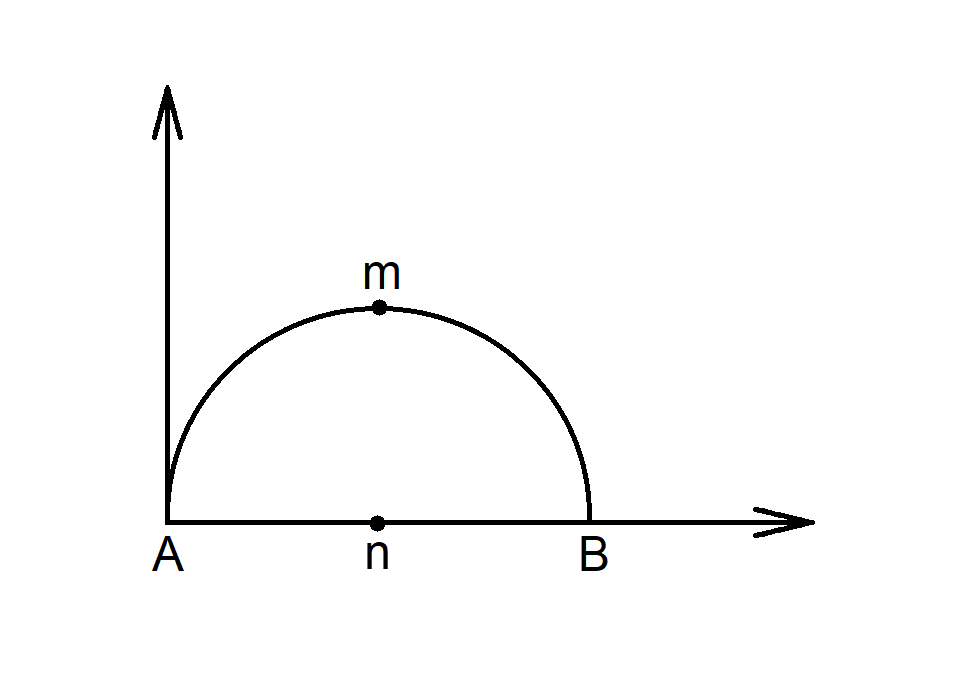
\includegraphics[scale = 0.5]{lec20_8.png}
	\end{center}
	Точки пересечения с осями: $A(0, 0), B(3, 0)$.
	
	\[
	\begin{gathered}
	\int\limits_{\tiny{\overbow{AB} \cup \overbow{BnA}}} x^2 \cos y\, dx
	- \frac{x^3}{3}	\sin y\, dy =
	\left[ \text{формула Грина} \right] =
	\iint\limits_{G} 0\, dx\, dy
	\implies
	\int\limits_{\tiny{\overbow{AB}}} =
	\int\limits_{\tiny{\overbow{AnB}}} = \\
	= \int\limits_{\tiny{\overbow{AnB}}} x^2 \cos y\, dx
	- \frac{x^3}{3}	\sin y\, dy =	
	\left[ 
		\overbow{AnB}:
		\left\{
		\begin{array}{l}
		y = 0 \\
		0 \leq x \leq 3
		\end{array}
		\right.
	\right] =
	\int\limits_{0}^{3} x^2\, dx = 9.
	\end{gathered}
	\]
\end{example}

\subsection{Вычисление площади с помощью КрИ}

Пусть требуется вычислить площадь области с границей $L$. 

Если взять $P(x, y)$ и $Q(x, y)$ такие, что
\[
Q_x'(x, y) - P_y'(x, y) = 1,\ \forall\, (x, y) \in G,
\]
то
\[
\int\limits_{L} P\, dx\, + Q\, dy = \iint\limits_{G}\, dx\, dy
= S = \mes G.
\]

Например:
	\begin{itemize}
		\item[a)] $ P(x, y) = 0,\ Q(x, y) = x $
		\item[б)] $ P(x, y) = -y,\ Q(x, y) = 0 $
		\item[в)] $ P(x, y) = -\dfrac{y}{2},\ Q(x, y) = \dfrac{x}{2}.$
	\end{itemize}

\[
S = \int\limits_{L} x\, dy =
- \int\limits_{L} y\, dx\, =
\frac{1}{2}\, \int\limits_{L} x\, dy - y\, dx.
\]

\begin{example}
	Пусть $\displaystyle
	\frac{x^2}{a^2}\, +\, \frac{y^2}{b^2}\, =\, 1$~--- уравнение границы $L$.
	
	\[
	\begin{gathered}
		S = \frac{1}{2}\int\limits_{L} x\, dy - y\, dx = 
		\left[
			\begin{gathered}
				x = a \cos t, \\
				y = b \sin t, \\
				0 \leq t \leq 2x
			\end{gathered}
		\right] =
		\frac{1}{2}\, \int\limits_{0}^{2\pi}\, \left( a \cos t\, b \cos t +
		b \sin t\, a \cos t \right) dt 
		= \frac{ab}{2}\, \int\limits_{0}^{2\pi}\, dt =
		\pi ab.
	\end{gathered}
	\]
\end{example}

\end{document}
